\section{Results}
\label{sec:10_5_results}



%%%%%%%%%%%%%%%%%%%%%%%%%%%%%%%%%%%
% Study infrastructure changing demand and cars
% unsatisfied trips
%%%%%%%%%%%%%%%%%%%%%%%%%%%%%%%%%%%


\begin{figure}[t]
\centering
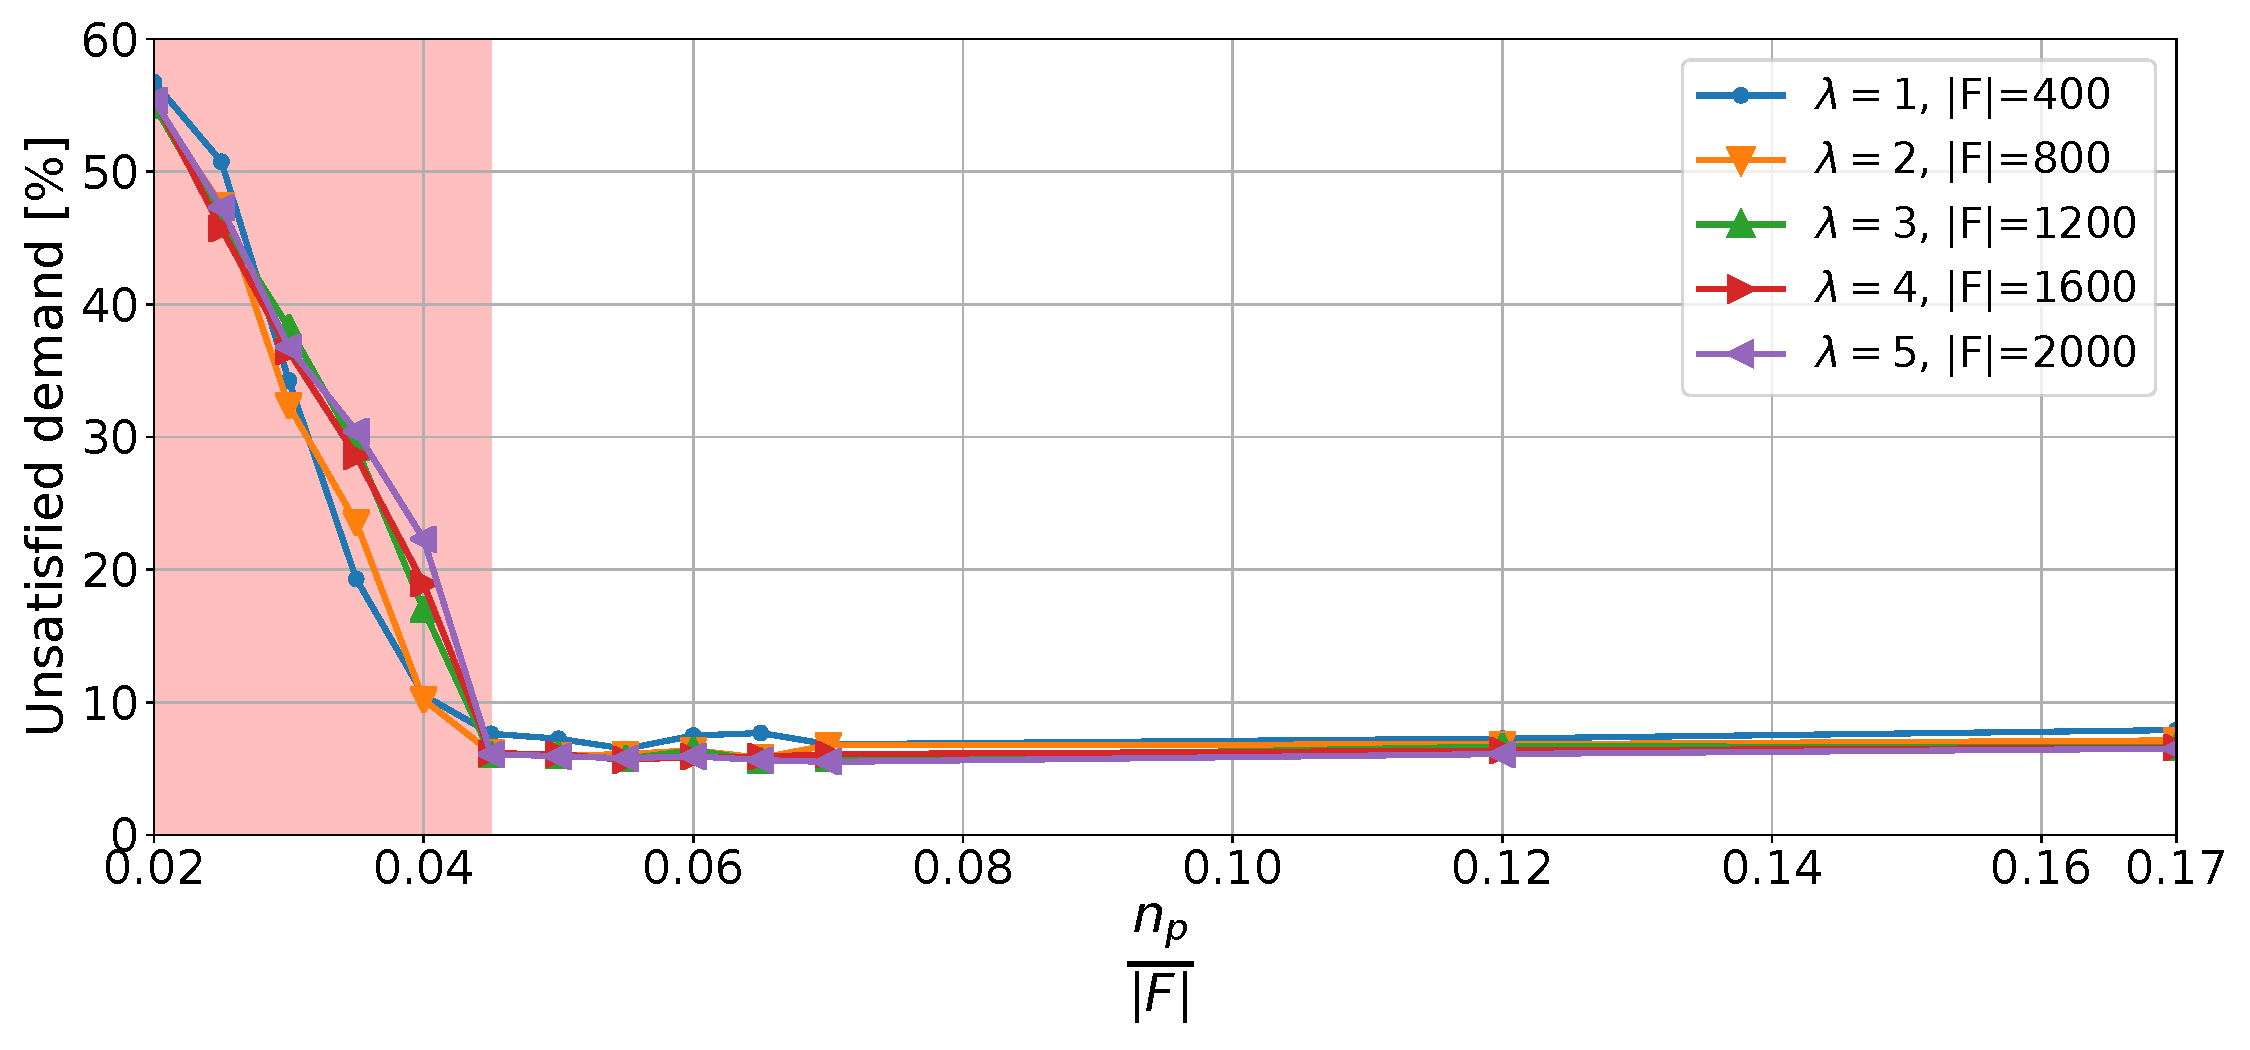
\includegraphics[width=1.\linewidth]{fig/final/unsatisfied_zp-5.pdf}
\caption{Unsatisfied demand with respect to different number of poles per vehicle. Curves show performance with different demand factor $\lambda$ and fleet size $|F|$, with $z_p$ = 0.05.}
\label{fig:10_5_unsatisfied_load1_zp5}
\end{figure}


\begin{figure}[t]
\centering
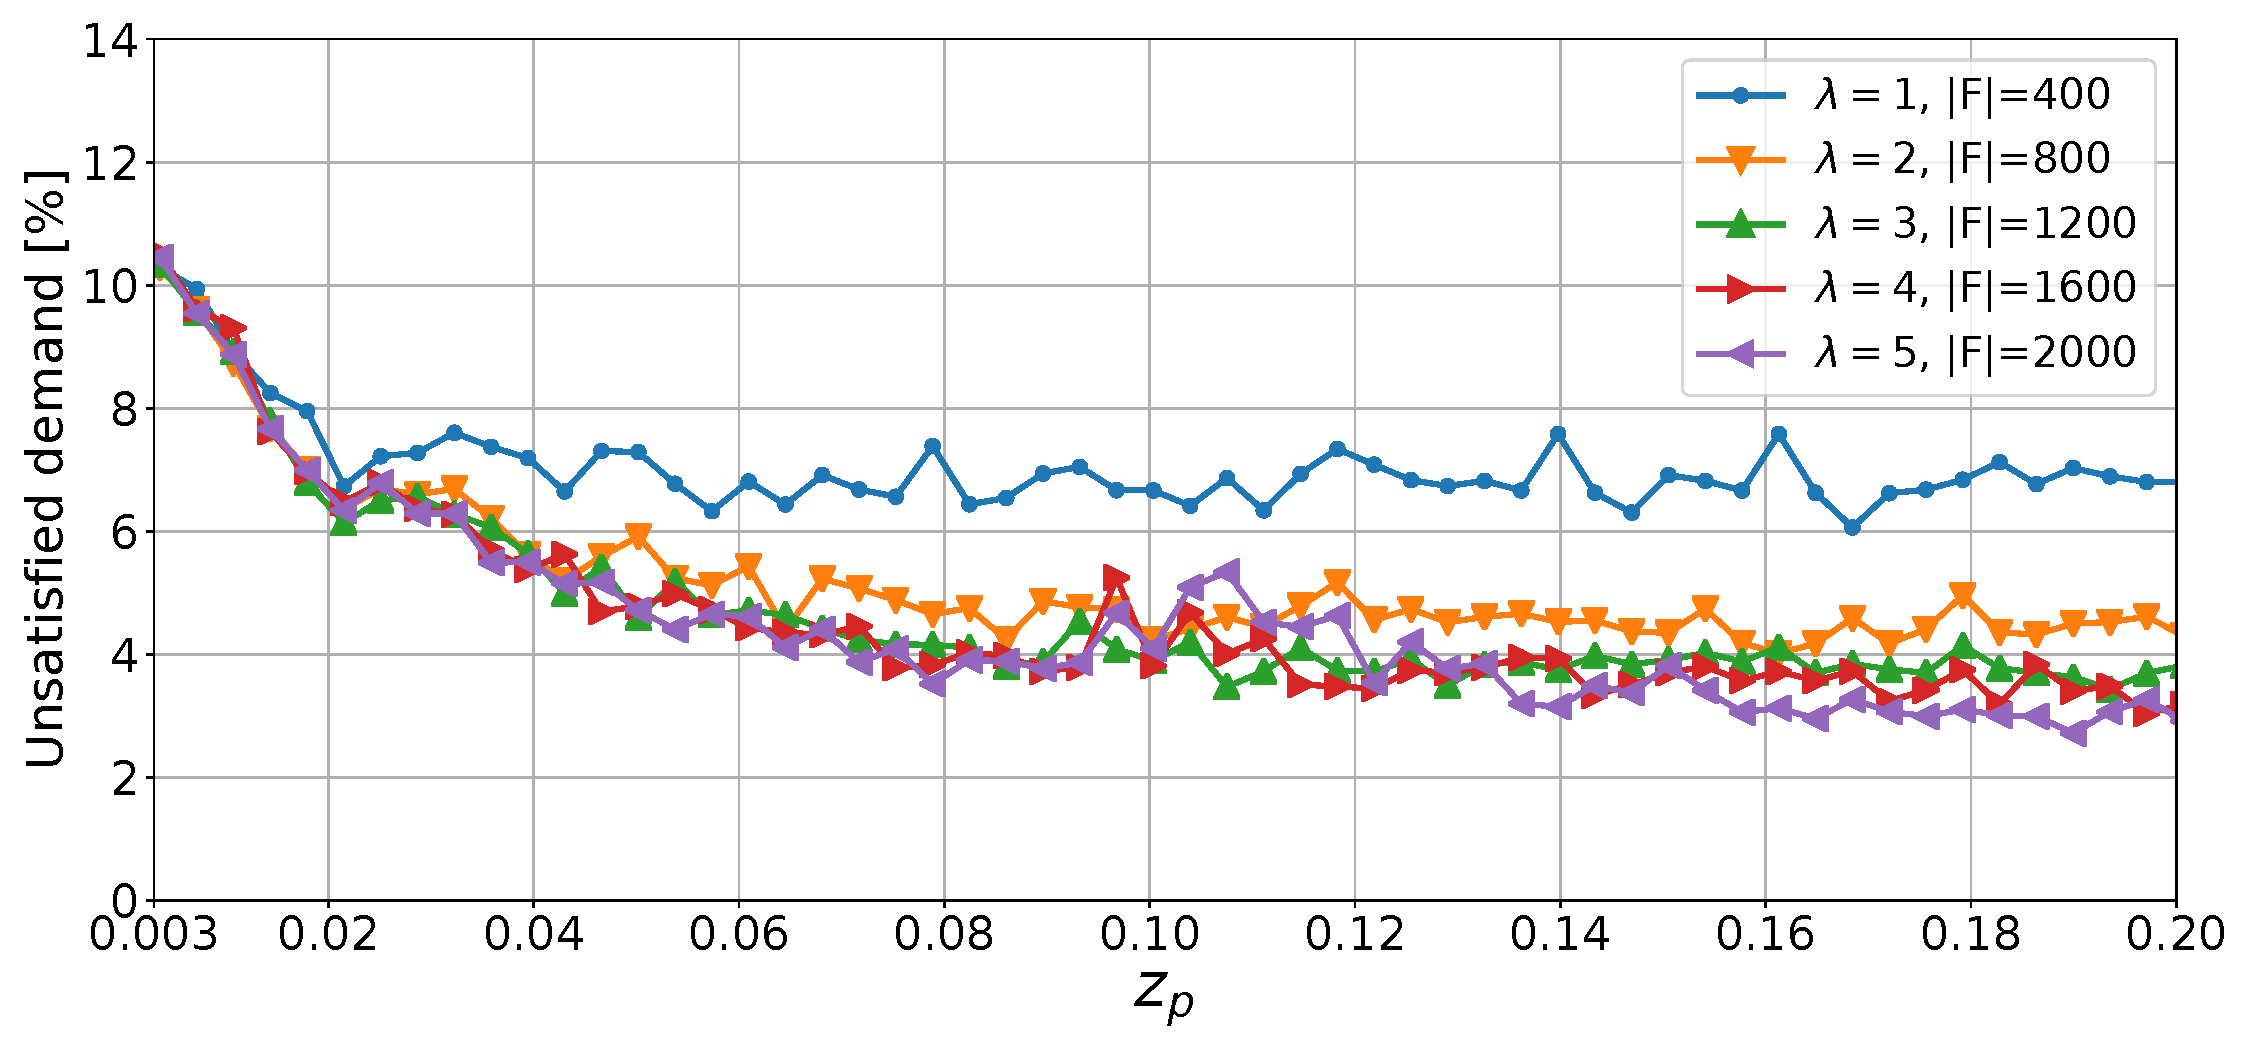
\includegraphics[width=1.\linewidth]{fig/final/unsatisfied_zp.pdf}
\caption{Unsatisfied demand with respect to the fraction of zones with charging poles  $z_p$. Curves show performance with different demand factor $\lambda$ and fleet size $|F|$, with  $n_p/|F|$ = 0.06.}
\label{fig:10_5_unsatisfied_zp}
\end{figure}

Given the multiple system design parameters, here we proceed by steps. First we analyse the impact on performance in order to select good design options. We then project the results through the cost figures to gauge the economic implications of these choices.

We consider as starting parameters the ones referring to the current FFCS running in Turin based on ICE cars, i.e., a fleet size $|F|=400$ and demand scaling factor $\lambda=1$. We explore the charging infrastructure design options, namely its size $n_p$ and extensiveness $z_p$. We fix $\alpha=0.25$ corresponding to the minimum energy needed to perform the longest trip in Turin~\cite{7_cocca2019free}.
We also check the impact of increasing the demand up to $\lambda=5$. Correspondingly, we increase the fleet size $|F(\lambda)|=400\cdot \lambda$ by the same factor. Each simulation considers three months of virtual time, corresponding to more than 200\,000 rental requests for $\lambda=1$.

\subsection{Impact of infrastructure design options}

Focus first on the impact of the number of poles per vehicles $n_p/|F|$ on the unsatisfied demand - reported in Figure~\ref{fig:10_5_unsatisfied_load1_zp5}. Consider $\lambda=1$ first. Here $z_p=0.05$ (14 charging zones). We observe two working regions: on the right - the charging infrastructure has enough capacity to supply the energy to support all customers' trips - resulting in a constant unsatisfied demand. On the left, system charging capacity goes below a minimum threshold (highlighted by the red area). Here the charging infrastructure cannot supply enough energy and unfeasible trips grow linearly with the lack of energy.
Consider now a demand factor that doubles ($\lambda=2$, and $|F|=2\cdot 400$). The energy supply must grow by a factor of 2 to supply twice the number of trips. As such the minimum threshold in terms of number of poles per vehicles remains the same. The same holds for higher $\lambda$.
Interestingly, the number of poles to supply the energy to cope with the mobility demand is quite small: a pole every 20 cars results enough.

There is still a 5-7\% of unsatisfied demand which results from the mismatch between zones with available cars, and zones with demand. We now check the impact of $z_p$ on this.
Figure~\ref{fig:10_5_unsatisfied_zp} fixes $n_p/|F|=0.06$, and shows the impact of concentrating or spreading them on few or more zones. On the leftmost case, we have the ``charging hub'' scenario, meaning that all poles are located in a single zone where all cars must be brought for charging. This solution creates a surplus of cars in the zone where the hub is, and a lack of cars in other zones. Unsatisfied demand then grows, calling for relocation policies.
Increasing $z_p$ has the benefit of spreading cars in the city\footnote{For $\lambda=1$ we can equip $n_p=24$ zone maximum ($z_p=0.09$), after which results do not change. Differences are due to simulation randomness.}. Having opted to place poles in $top\_{park}$ zones, cars get naturally located there, facilitating customers that look for a car in those high-demand zones. This reduces the percentage of unsatisfied demand significantly, questioning the need of costly relocation policies. Performance-wise, the higher the fraction of zones with poles, the better.



\begin{figure}
\centering
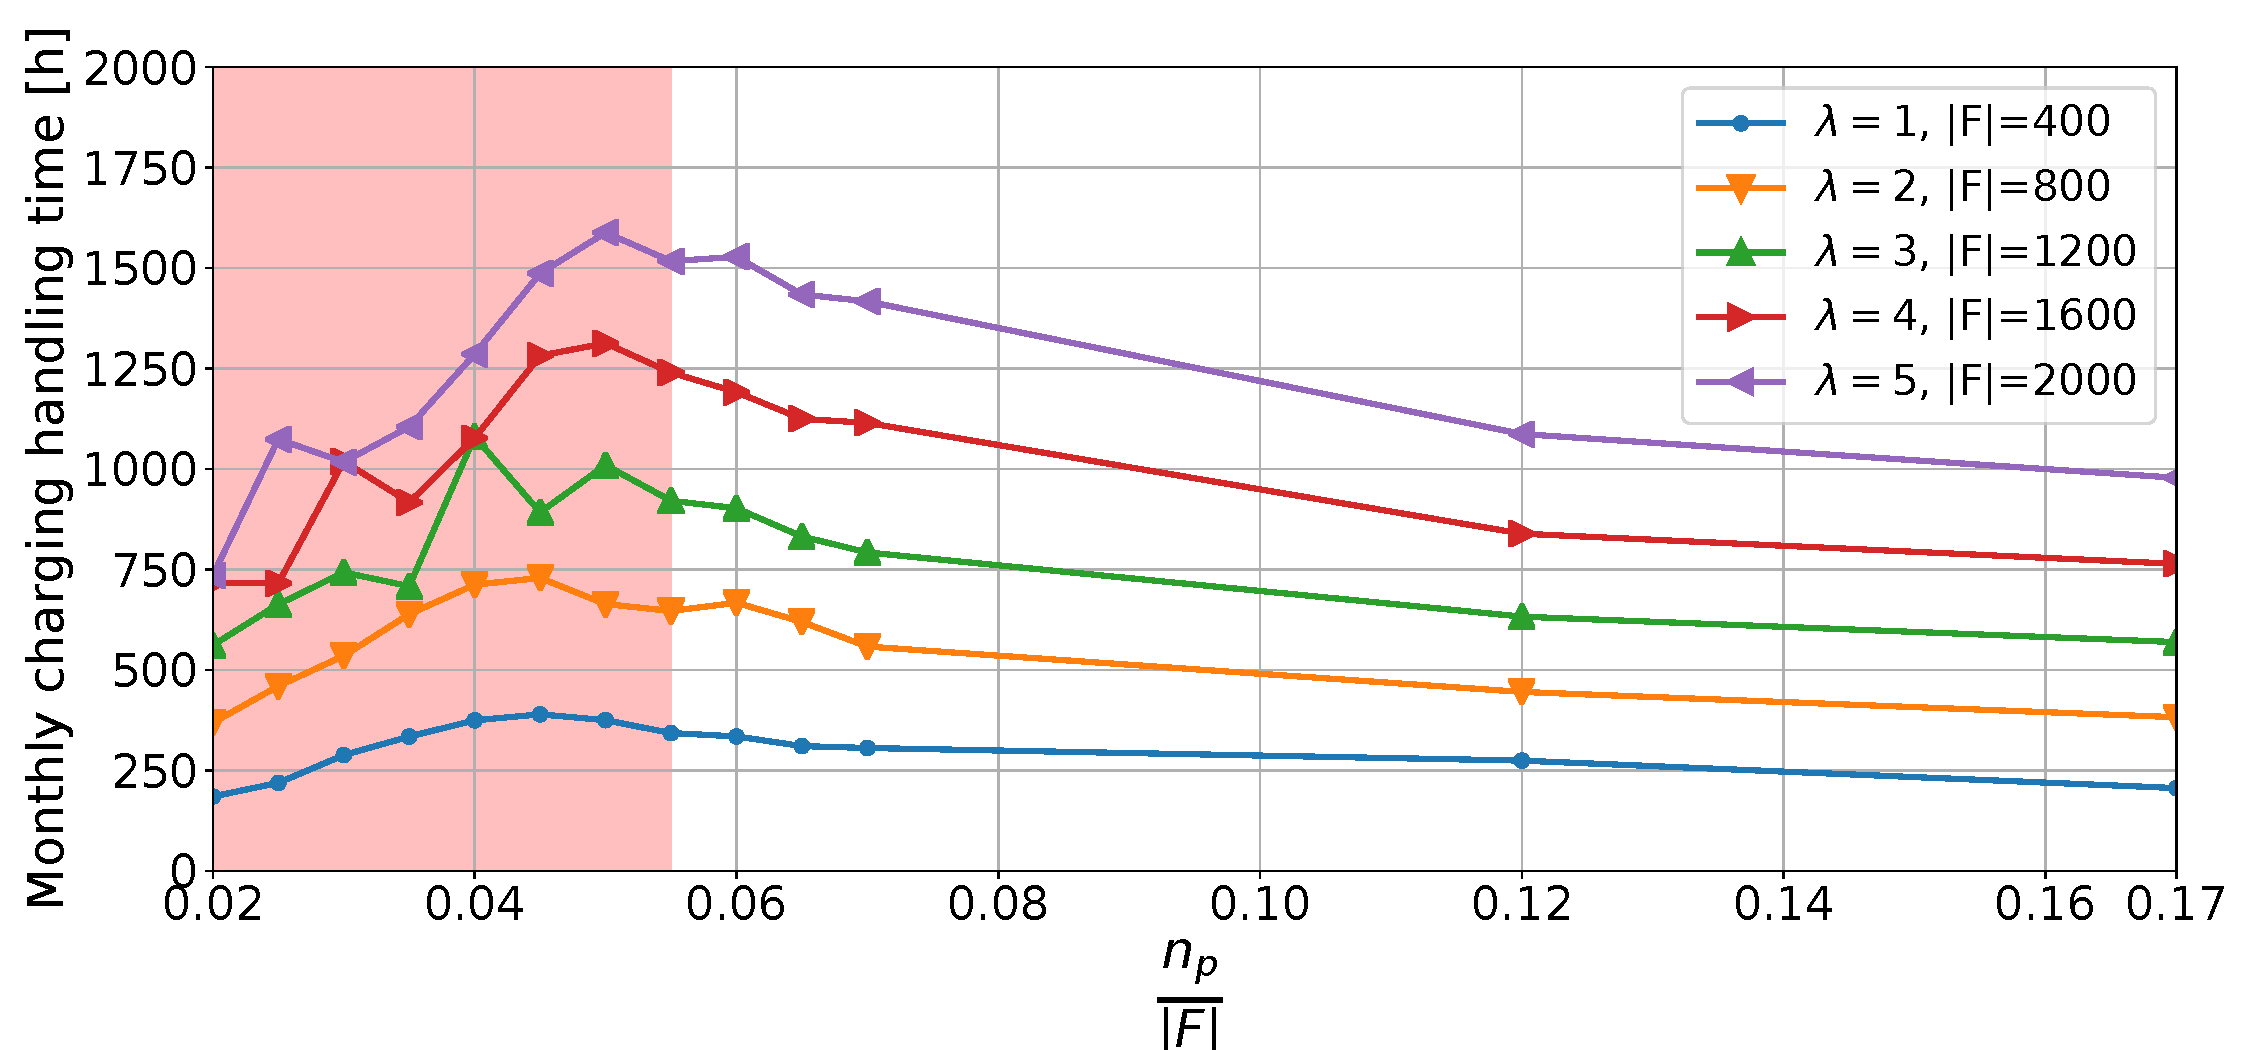
\includegraphics[width=1.\linewidth]{fig/final/relocost_zp-20.pdf}
\caption{Monthly charging handling time drivers have to spend to bring cars to charging poles. Curves show performance with different values of demand factor $\lambda$ and fleet size $|F|$, with $z_p=0.20$.}
\label{fig:10_5_zp_relocost}
\end{figure}

\begin{figure}
\centering
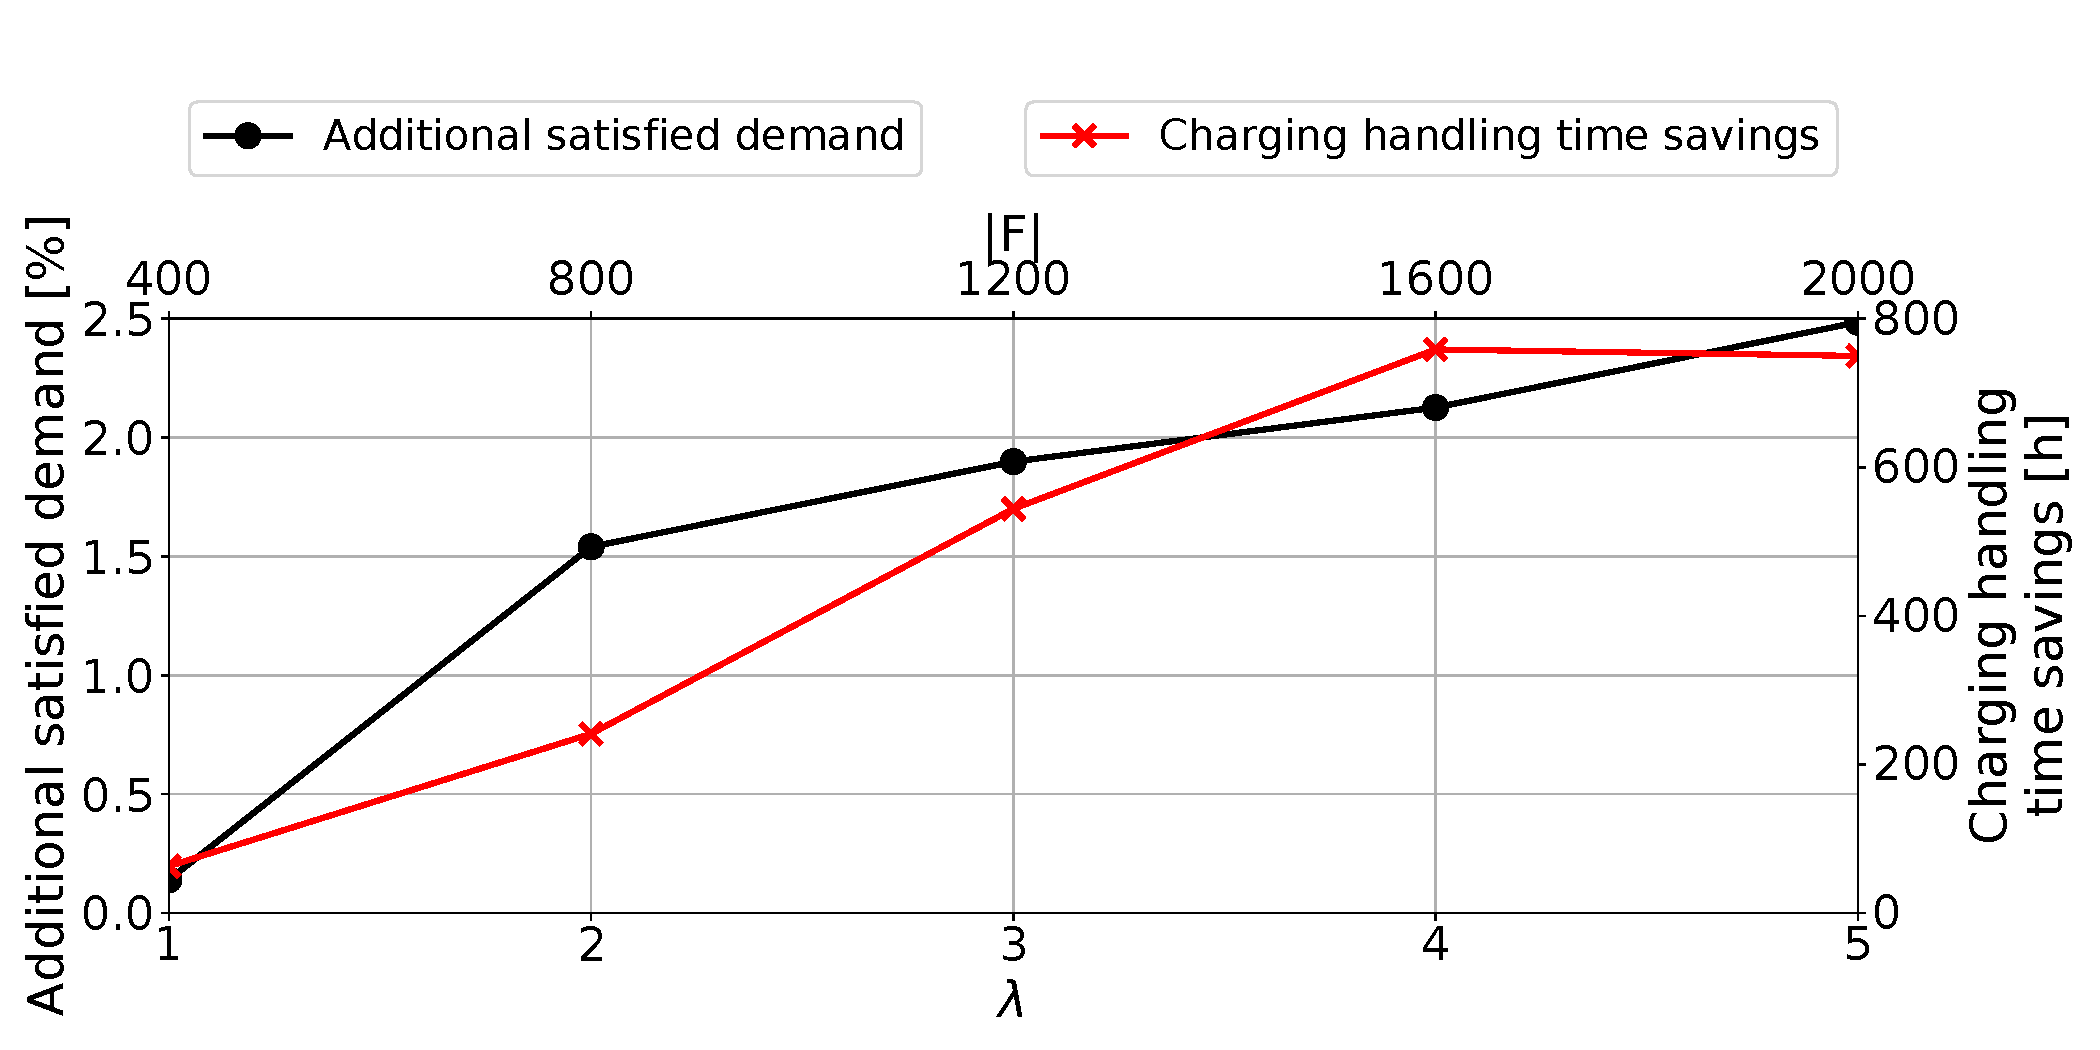
\includegraphics[width=1.\linewidth]{fig/final/zp_gain.pdf}
\caption{Gain in terms of satisfied demand and charging handling time of a more spread infrastructure ($z_p = 0.20$) with respect to a more centralized infrastructure ($z_p = 0.05$). Gain is showed for increasing demand factor $\lambda$ and fleet size $|F|$. Here $n_p/|F|$ = 0.06.}
\label{fig:10_5_zp_gain}
\end{figure}

Focus now on the time the system has to spend to bring cars to the closest charging pole, reported in Figure~\ref{fig:10_5_zp_relocost} for $z_p=0.20$. 
Notice that if the system cannot supply enough energy to satisfy the demand ($n_p/|F|<0.055$ in this case), the charging handling cost decreases. Likely not a good design choice being this due to loss of satisfied demand.
Consider the region $n_p/|F|\geq 0.055$, where the system has enough charging capacity. If there are just enough poles, most of them results busy, and the workers need to drive cars to far away free poles. This results in an increase of handling time up to 1600\,$h$ for $\lambda=5$. By increasing $n_p/|F|$, we increase the probability of finding a nearby free pole, shortening handling time down to 1000\,$h$ per  month for $\lambda=5$.
As expected, the higher $\lambda$, the higher the time to handle charging events -- with an almost perfect linear increase.

This highlights a trade-off between infrastructure costs and management costs. To better gauge this, Figure~\ref{fig:10_5_zp_gain} compares a more concentrated system with $z_p=0.05$ with a more distributed system with $z_p=0.20$. We plot the "additional satisfied demand" (black curve) and the saving in charging handling time (red curve) for increasing demand factor $\lambda$ and fleet size $|F|$ (fixing $n_p/|F|$ = 0.06). In all cases, $z_p=0.20$ results in higher satisfied demand and lower cost than $z_p=0.05$, with benefits that increase with increasing demand. In a nutshell, distributing the same number of poles among more zones improves system performance and reduces charging handling time. Clearly this needs to be weighted by the additional cost of installing a more distributed charging infrastructure.

\subsection{Impact of fleet size}
We now explore the impact of the number of cars when the demand increases. For this, we scale $\lambda$, but keep the fleet size constant to $|F|=400$. For simplicity, we consider a  charging infrastructure capacity that can cope with the highest demand, i.e., $n_p=120$. We consider two cases, $z_p=0.05$ and $z_p=0.20$. We plot results in Figure~\ref{fig:10_5_unsatisfied_zp_fixed_request}.
Interestingly, the same number of vehicles can sustain a sizeable increase in $\lambda$ without a significant impact the unsatisfied demand. 
For instance, $|F|=400$ vehicles can cope with a factor $\lambda=3$ increase in the demand, just losing 2.5\% of customer requests. This would result in a significant saving in the cost of vehicles. Given there are no differences in concentrating or spreading the charging poles in few or more zones, we fix $z_p=0.20$ from now on.

\begin{figure}
\centering
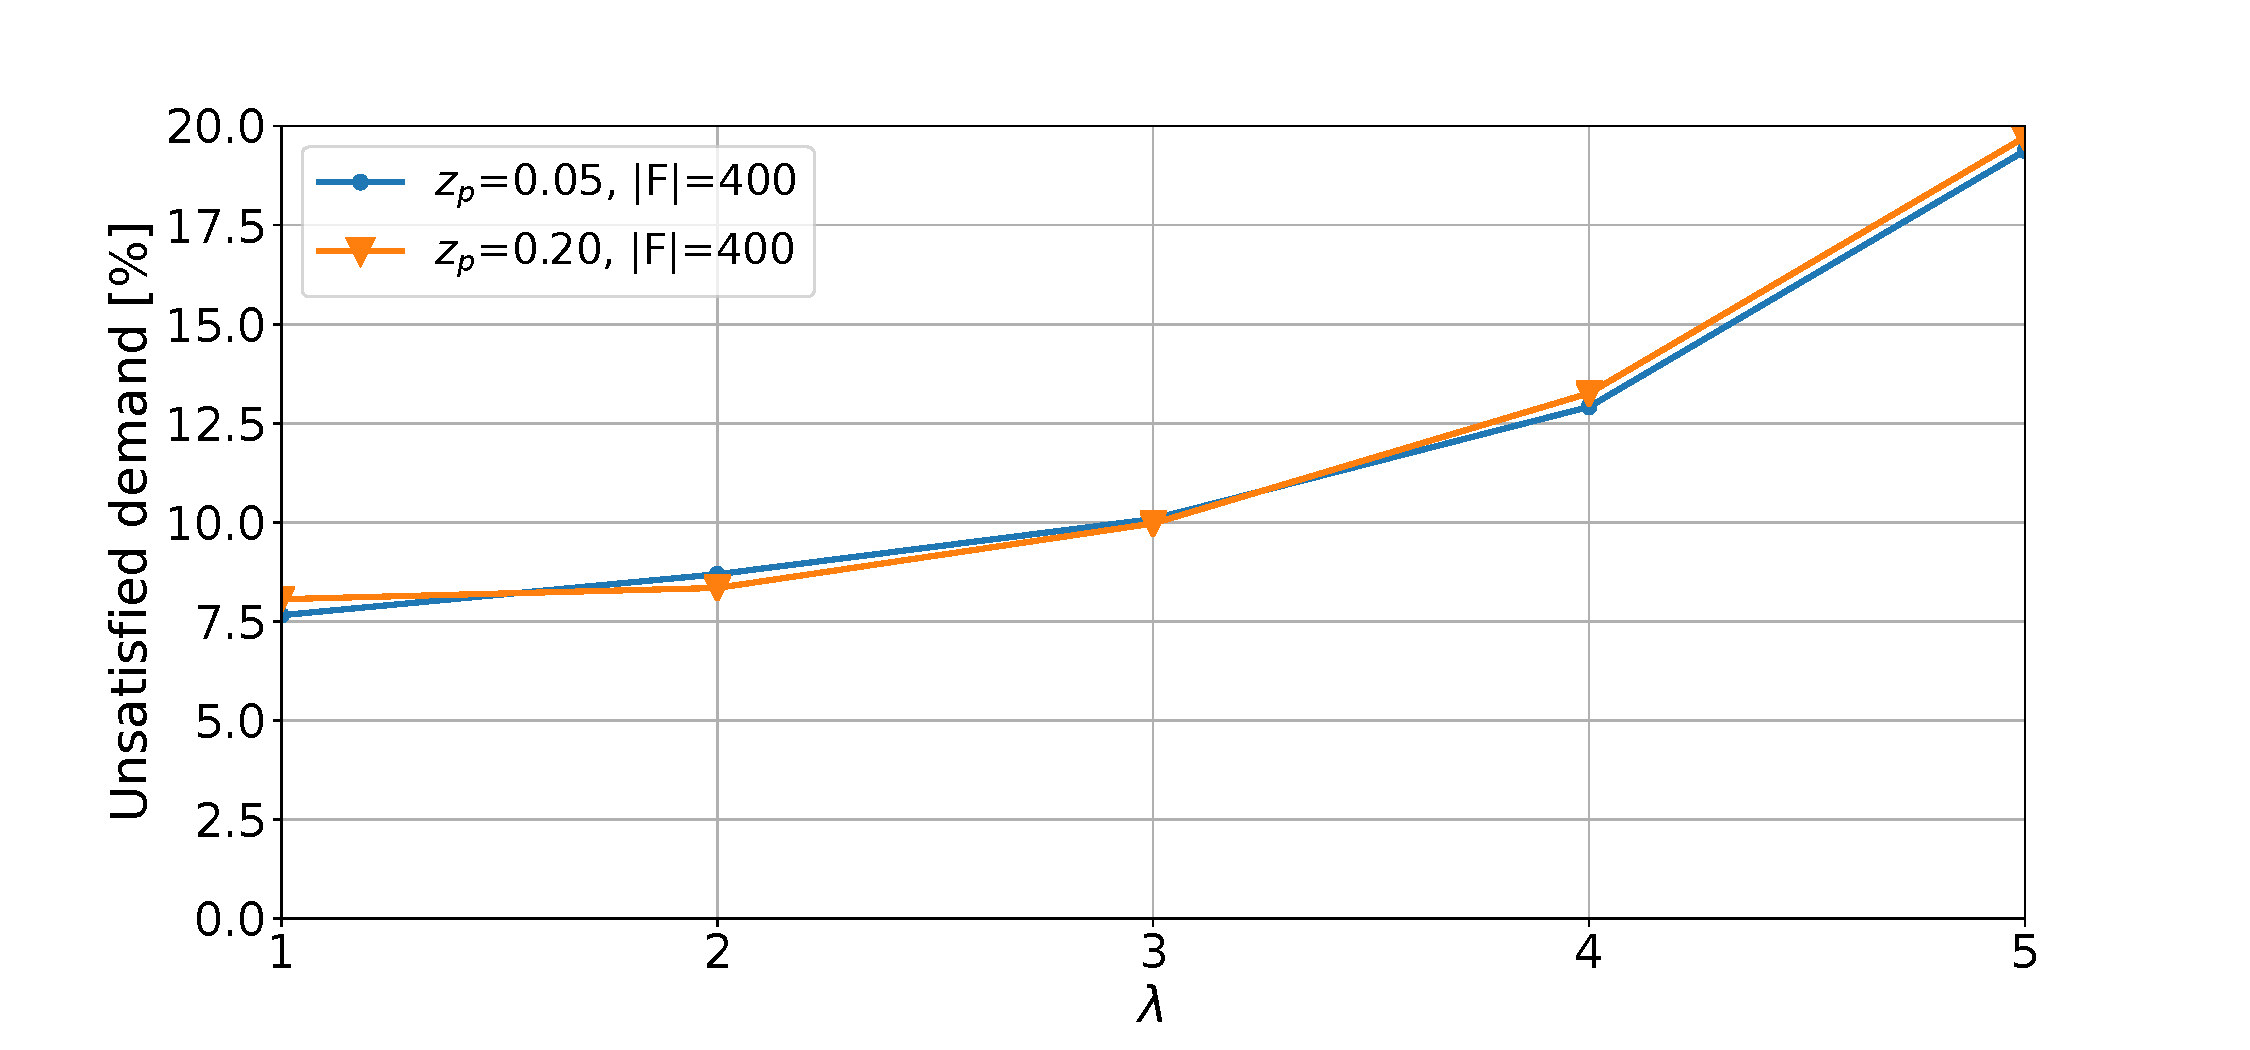
\includegraphics[width=1.\linewidth]{fig/final/const_fleet_zp.pdf}
\caption{Unsatisfied demand for increasing values of $\lambda$ but same number of vehicles $|F|=400$, and large enough charging infrastructure ($n_p=120$).}
\label{fig:10_5_unsatisfied_zp_fixed_request}
\end{figure}

To observe how the unsatisfied demand would be impaired by further reducing the number of cars and/or the number of poles, we present contour maps in Figures~\ref{fig:10_5_contour_unsatisfied_rate-1} and Figure~\ref{fig:10_5_contour_unsatisfied_rate-5}, for $\lambda=1$ and $\lambda=5$, respectively. 
Interestingly, the two design parameters seem to affect unsatisfied demand in almost independent manner. On the one hand, reducing the number of cars has limited impact until we reach very small values. For instance, halving the fleet size down to $|F|=200$ would increase the unsatisfied demand by 6-8\% only.
On the other hand, increasing $n_p$ brings no benefit - provided there are enough poles (cfr. Figure~\ref{fig:10_5_unsatisfied_load1_zp5}).


\begin{figure}[ht]
	\begin{subfigure}{0.5\textwidth}
		\centering
		% include first image
		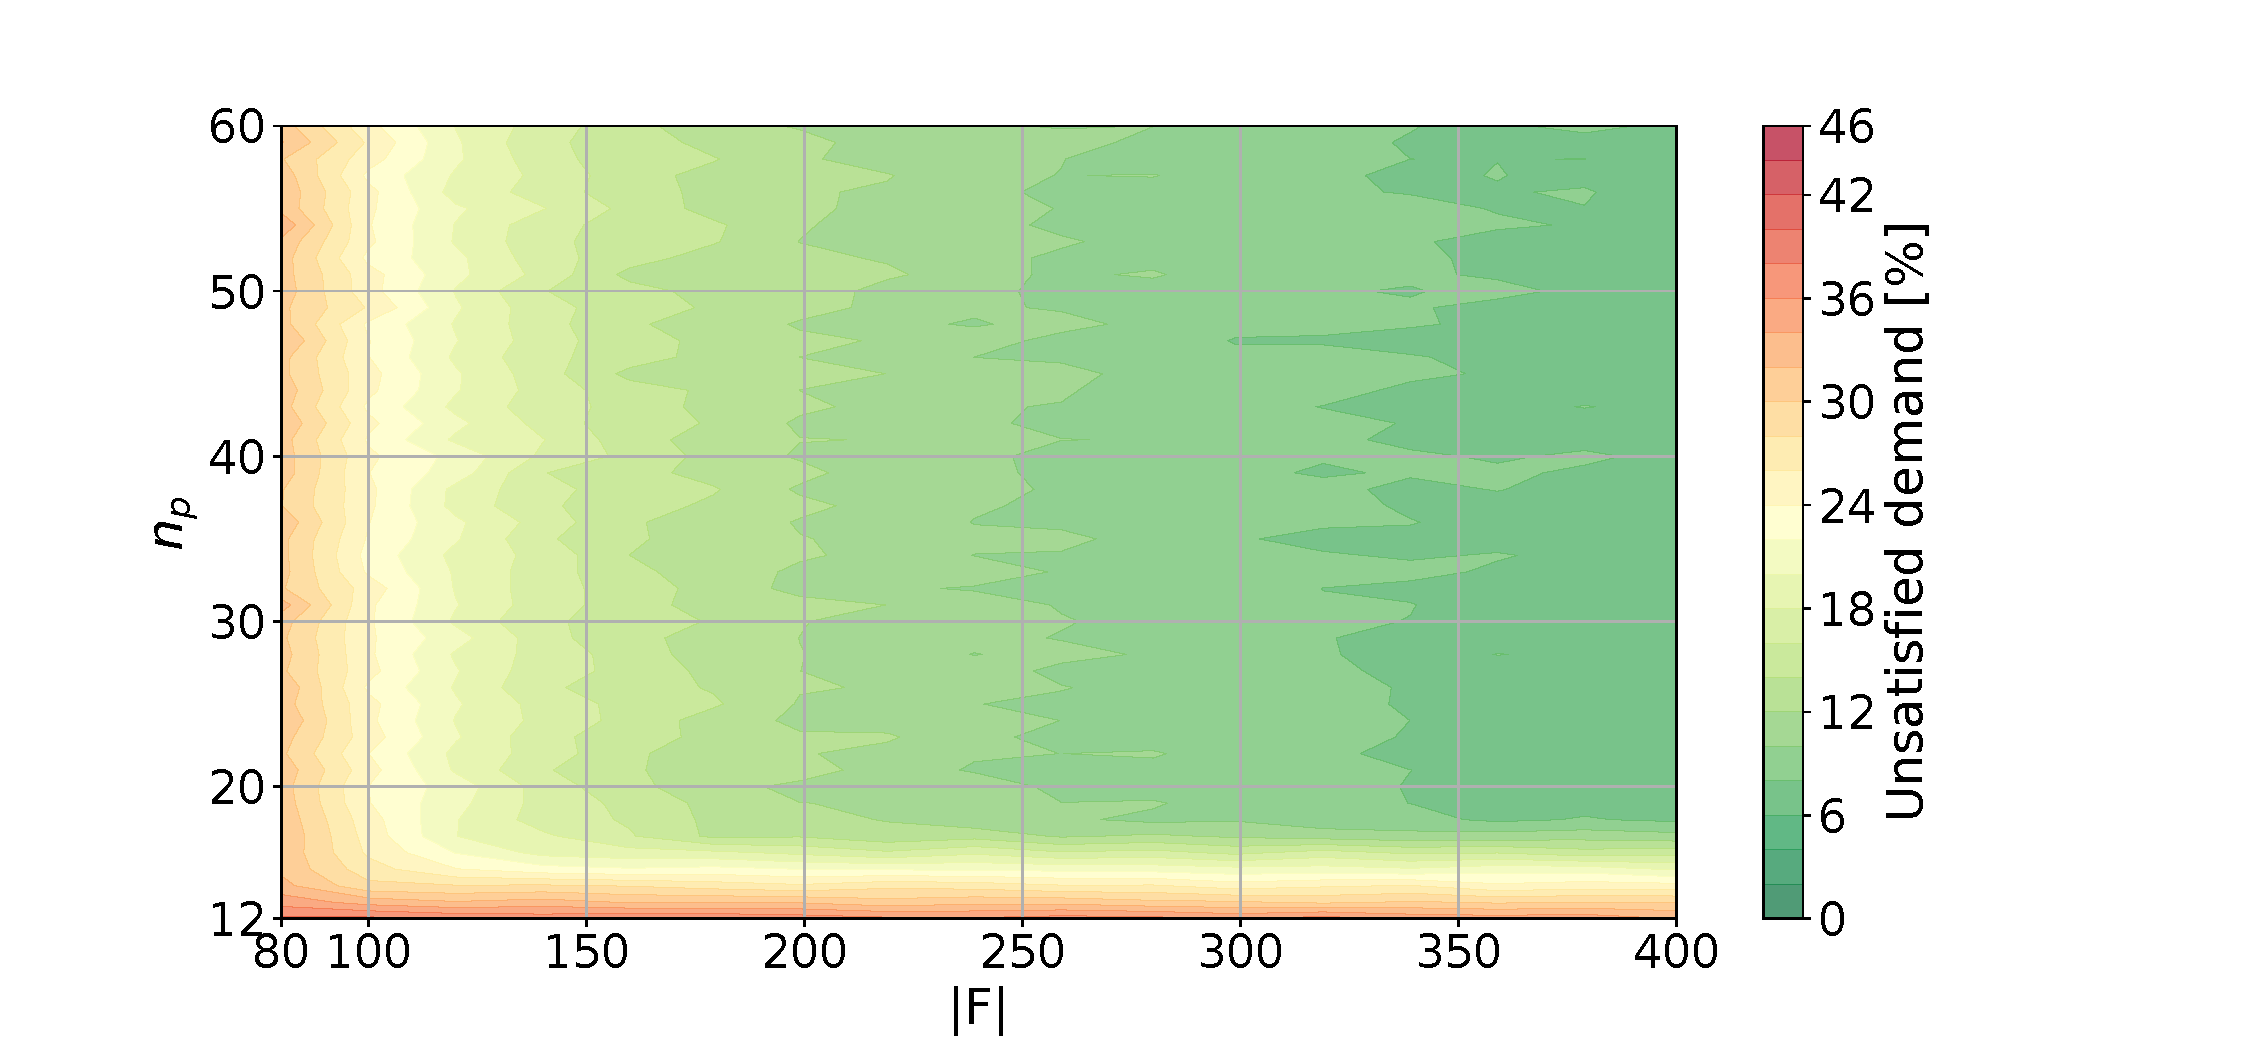
\includegraphics[width=1\linewidth]{fig/final/contour_unsatisfied_rate-1.pdf}  
		\caption{Demand factor $\lambda=1$}
		\label{fig:10_5_contour_unsatisfied_rate-1}
	\end{subfigure}
	\begin{subfigure}{0.5\textwidth}
		\centering
		% include second image
		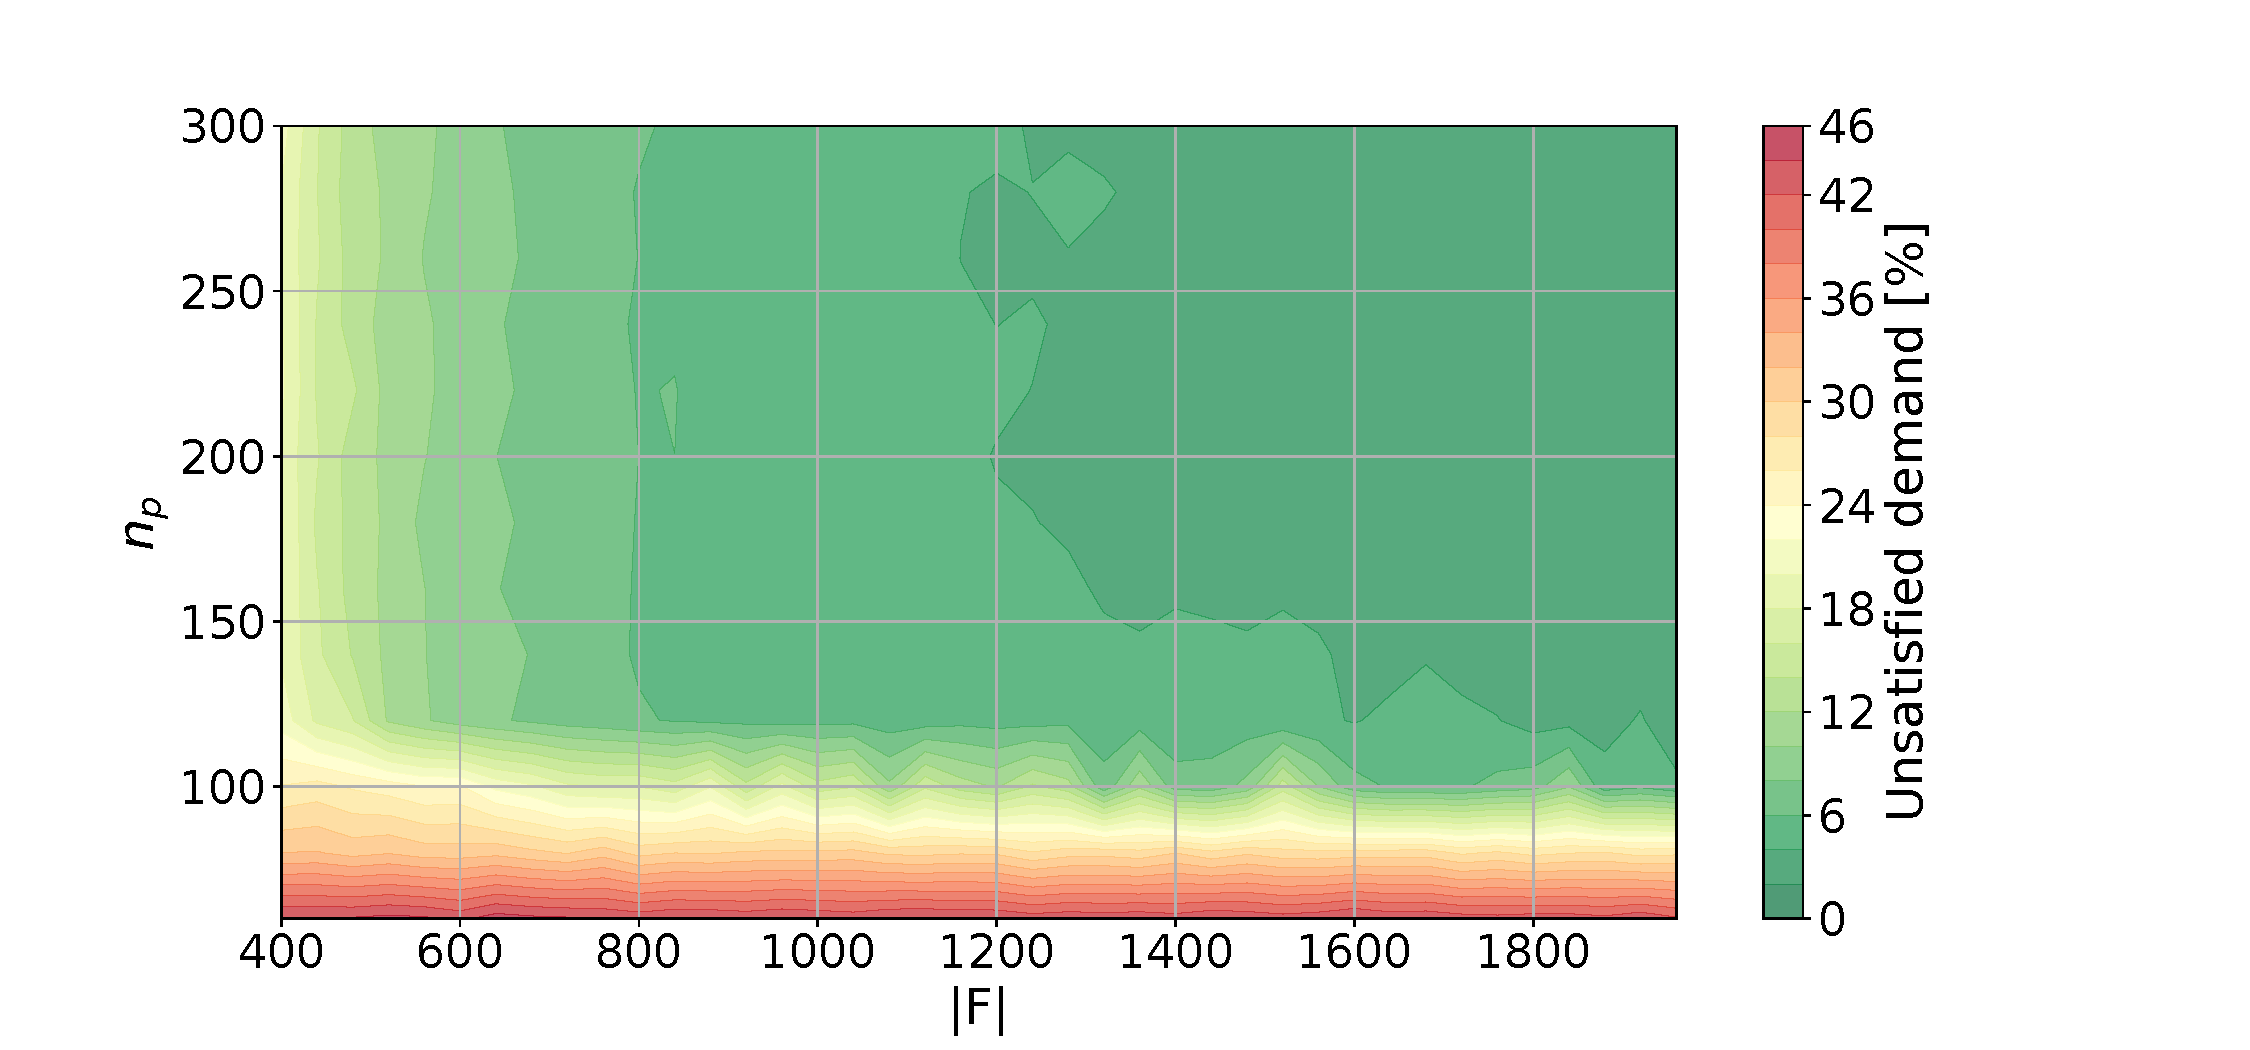
\includegraphics[width=1\linewidth]{fig/final/contour_unsatisfied_rate-5.pdf}  
		\caption{Demand factor $\lambda=5$}
		\label{fig:10_5_contour_unsatisfied_rate-5}
	\end{subfigure}
	\caption{Unsatisfied demand varying number of poles $n_p$ and fleet size $|F|$ with $z_p=0.20$.}
	\label{fig:10_5_contour_unsatisfied_rate}
\end{figure}

\begin{figure}[ht]
	\begin{subfigure}{0.5\textwidth}
		\centering
		% include first image
		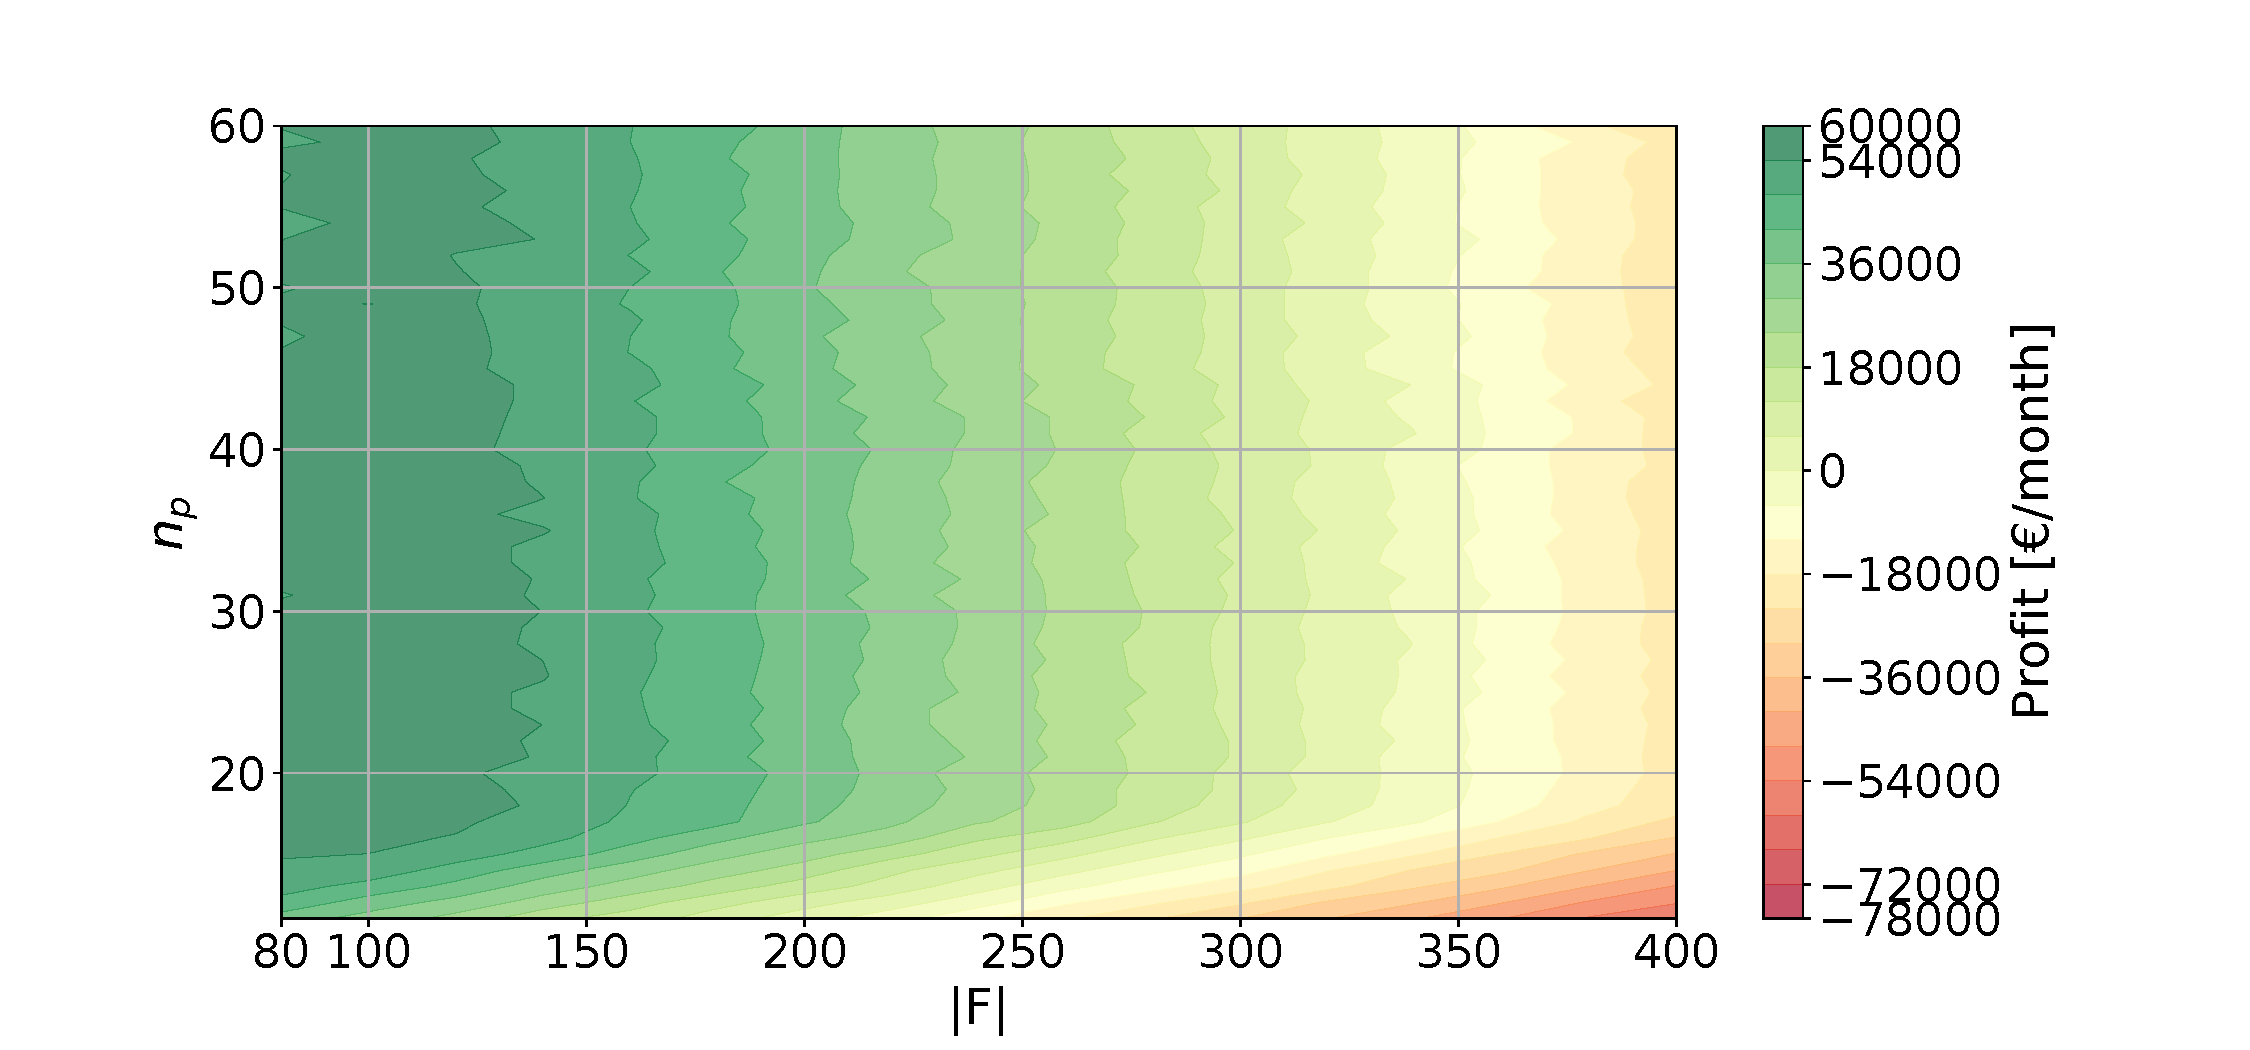
\includegraphics[width=1\linewidth]{fig/final/contour_profit_rate-1.pdf}  
		\caption{Demand factor $\lambda=1$}
		\label{fig:10_5_profits_rate-1}
	\end{subfigure}
	\begin{subfigure}{0.5\textwidth}
		\centering
		% include second image
		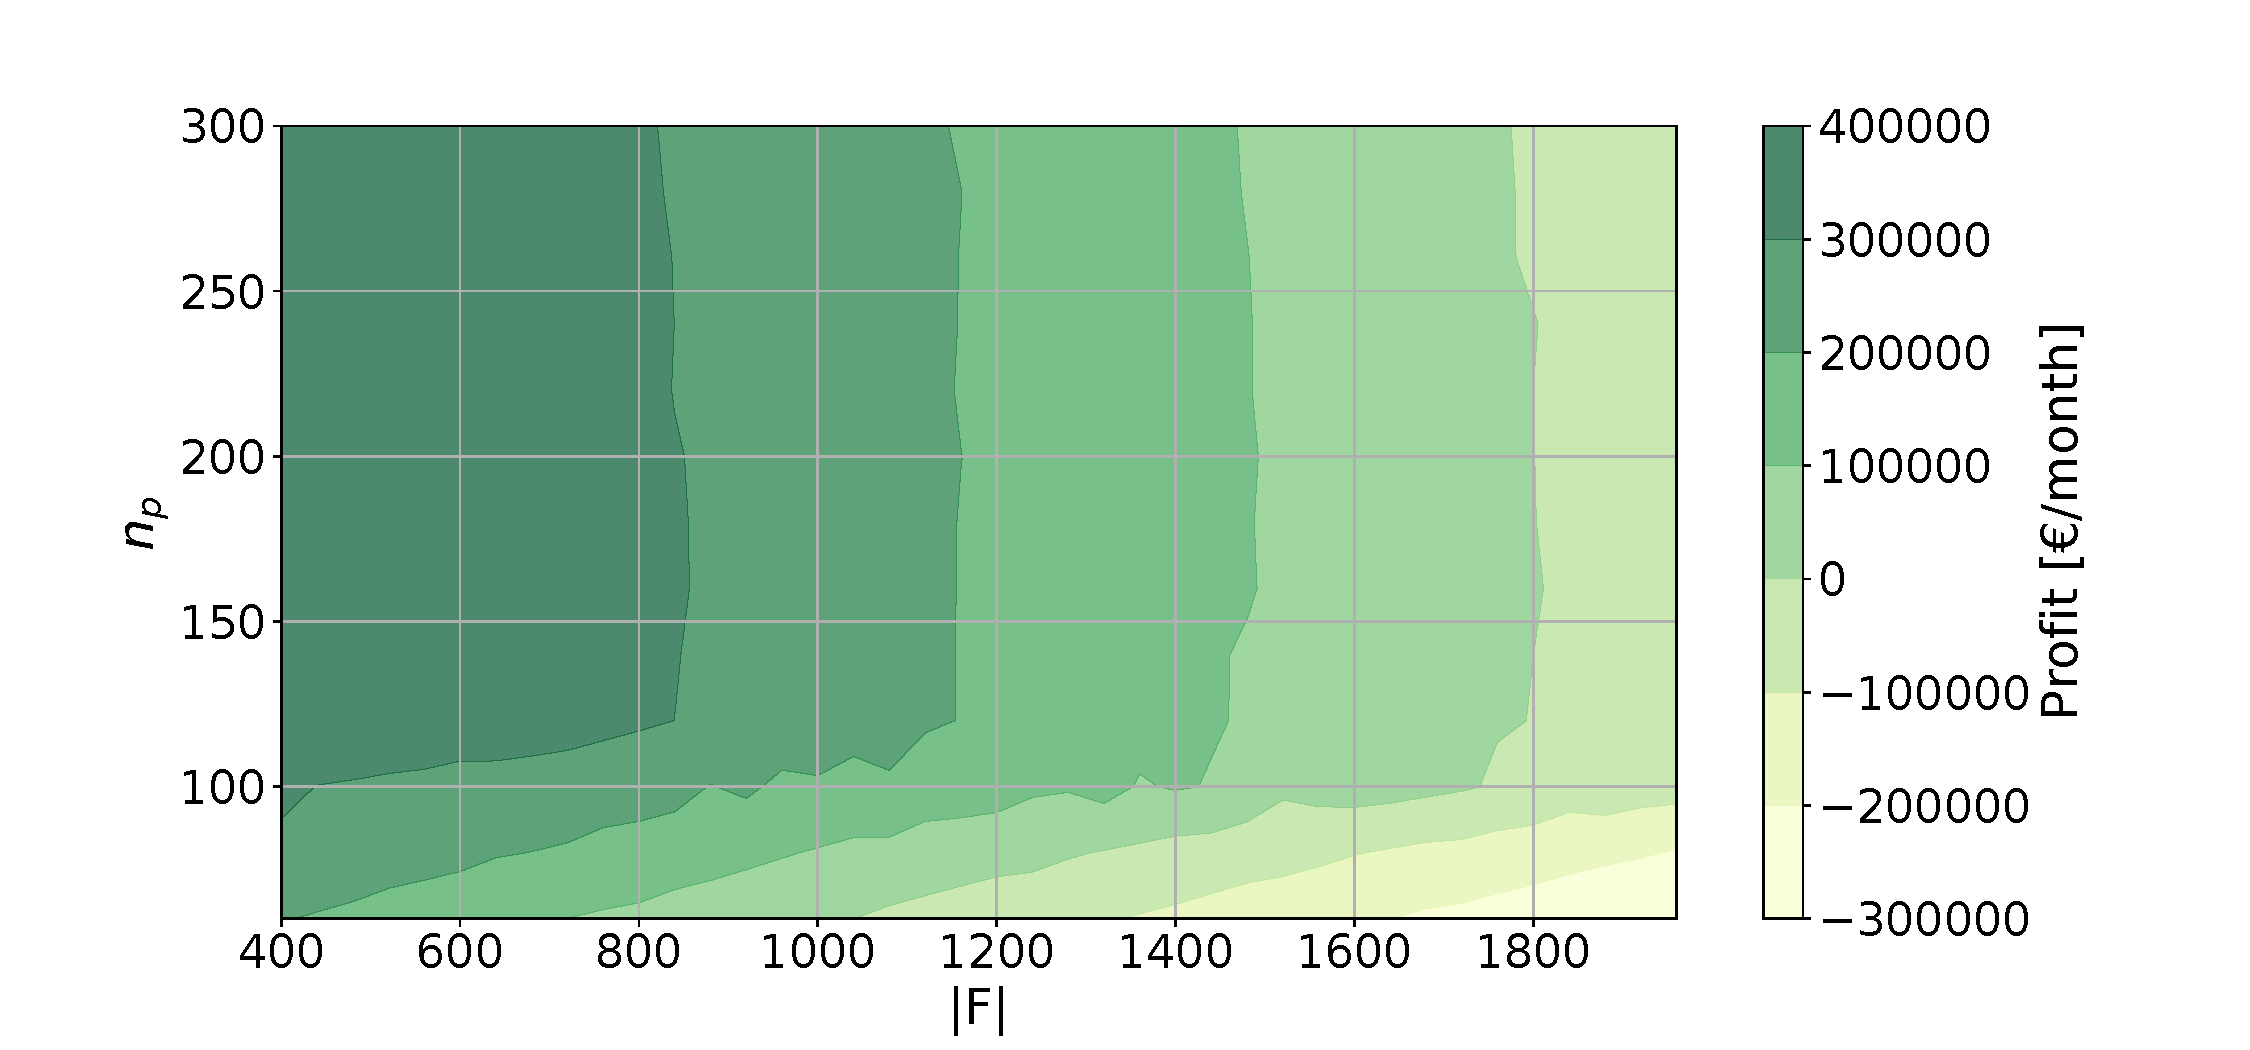
\includegraphics[width=1\linewidth]{fig/final/contour_profit_rate-5.pdf}  
		\caption{Demand factor $\lambda=5$}
		\label{fig:10_5_profits_rate-5}
	\end{subfigure}
	\caption{Monthly estimated profits varying number of poles $n_p$ and fleet size $|F|$ with $z_p=0.20$.}
	\label{fig:10_5_profits_rate}
\end{figure}



The same considerations hold when $\lambda=5$, with a slightly higher interaction between $n_p$ and $|F|$ when approaching small values for both. Observe also a large region with unsatisfied demand lower than 6\% (dark green). The high number of vehicles allows a high multiplexing gain so that fewer cars can offer the same service level. For instance, $|F|=800$ cars guarantee about 10\% of unsatisfied demand if $n_p>120$. In a nutshell, the system needs less cars to satisfy the same percentage of demand when the demand increases, with significant economy of scale gain.


\subsection{Impact of costs}


%It is quite a result because we can face a quintupled demand doubling our fleet. Indeed, there seems to be a value for the number of poles that guarantees that specific fraction of unsatisfied users. After reaching this number of poles if we keep on increasing one of the two parameters we can not appreciate any differences in terms of this performance metric. 



%%%%%%%%%%%%%%%%%%%%%%%%%%%%%%%%%%%
% Study vehicles and poles
% costs and revenues
%%%%%%%%%%%%%%%%%%%%%%%%%%%%%%%%%%%


To have a clear and complete picture, we now project the performance indexes into economic figures. Here we compare the monthly profit an EVs FFCS provider would reach for different combinations of the number of vehicles and the number of poles, i.e., its investment in the fleet and charging infrastructure. All costs included in Table~\ref{tab:summary} are considered.

Figure~\ref{fig:10_5_profits_rate-1} shows the results for $\lambda=1$. Green shades reflect positive profit, while yellow and red shades highlight loss-making configurations. Interestingly, the zones with the highest profits tend to be in the leftmost part of the figure, i.e., for small number of cars. While this causes a higher unsatisfied demand - see Figure~\ref{fig:10_5_contour_unsatisfied_rate-1} - it looks the only way to reduce the cost of the fleet so to have a profitable system. The impact of the charging infrastructure is quite negligible unless when $n_p$ becomes too small (i.e., when not enough charging capacity is present). This is due to the low cost of buying and installing a charging pole when amortized on $p_{life}=10$ years. Recall that we have seen that the charging infrastructure design calls for a charging pole every 20 vehicles. As such, the overall economic impact of the charging infrastructure results quite negligible compared to the fleet size costs.

The picture improves drastically when $\lambda=5$, shown in Figure~\ref{fig:10_5_profits_rate-5}. Here, we explore scenarios with a 5-fold increase in both the number of poles ($n_p\in[50,300])$, and in the number of vehicles ($|F|\in[400,2000]$) with respect to the $\lambda=1$ scenario. Here, all configurations result in positive profit. Even more interestingly, by reducing the number of cars we observe a marginal decrease in the profit, with the best scenarios being in $|F|\in[1400, 2000]$. This is due to large multiplexing effect we already observed in Figure~\ref{fig:10_5_unsatisfied_zp_fixed_request}. Even when reducing the number of cars to 800, we observe sizeable profits.

Considering the number of poles, as expected, when $n_p<120$ (the minimum threshold for constant unsatisfied demand when $|F|=2000$, showed in Figure~\ref{fig:10_5_unsatisfied_load1_zp5}) the insufficient system charging capacity impairs cars availability, increasing the unsatisfied demand. 
As seen already, increasing $n_p$ above the minimum threshold brings little benefit, but it also has little impact on the profits (due to the relatively low cost of pole installation). 

In summary, we can conclude that the FFCS provider needs to carefully evaluate the minimum number of poles when designing and implementing the charging infrastructure. The limited cost of pole installation, and the long amortization time make overprovisioning the charging infrastructure a viable option to make the system robust to demand increase.
Considering the fleet size, when the demand is low, the high cost of vehicles suggests limiting the number of vehicles. When instead the demand grows, an economy of scale gain is possible, making the system even profitable with large fleet size.





